\documentclass[12pt, a4paper]{article}
\usepackage{a4wide}

\usepackage[utf8]{inputenc}
\usepackage[spanish]{babel}

\usepackage{color}
\usepackage{url}
\definecolor{lnk}{rgb}{0, 0, 0.4}
\usepackage[colorlinks = true, linkcolor = lnk, citecolor = black,urlcolor = black]{hyperref}

\usepackage{./otros/ulem}
\usepackage{./otros/caratula}

\usepackage{amssymb}
\usepackage{pdfpages}
\usepackage{framed}

\usepackage[small, bf, labelformat = empty]{caption}	
\usepackage{subfig}
\usepackage{float}

\usepackage{makeidx}
\makeindex

\begin{document}
  %Carátula
	\titulo{Trabajo Práctico 1}
	\subtitulo{}
	\fecha{24 de Abril de 2013}
	\materia{Bases de Datos}
	\integrante{Agustina Ciraco}{630/06}{agusciraco@gmail.com}	
	\integrante{Nadia Heredia}{589/08}{heredianadia@gmail.com}
	\integrante{Pablo Antonio}{290/08}{pabloa@gmail.com}
	\integrante{Vanesa Stricker}{159/09}{vanesastricker@gmail.com}  
	\maketitle

	% Índice
	\small
	\newpage \printindex \tableofcontents
	\normalsize

	\newpage
	\section{Introducci\'on}

En este trabajo pr\'actico, analizaremos el impacto de las diferentes
estrategias para manejar los buffer pools.
Nos concentraremos en el m\'odulo \textit{Buffer Manager}.

\vspace*{0.3cm}

Las diferentes estrategias que consideraremos son

\begin{itemize}
    \item
            un solo buffer
    \item
            múltiples buffers (distribución de Oracle)    
\end{itemize}

\vspace*{0.3cm}

Veremos las ventajas y desventajas de cada uno seg\'un la situaci\'on.

\subsection{Formato}

\vspace*{0.3cm}

En primera instancia, presentaremos una breve explicación
del uso de los múltiples buffer, luego se explicar\'an ciertos 
detalles de implementaci\'on, as\'i como tambi\'en las decisiones 
tomadas durante el desarrollo.

\vspace*{0.3cm}

Por \'ultimo, daremos nuestras conclusiones.


	\newpage
	\section{Diagrama Entidad-Relaci\'on}

% -----------------------------------------------------------------------------
\thispagestyle{empty}
  \begin{figure}[H] \centering
    \subfloat[der]
    {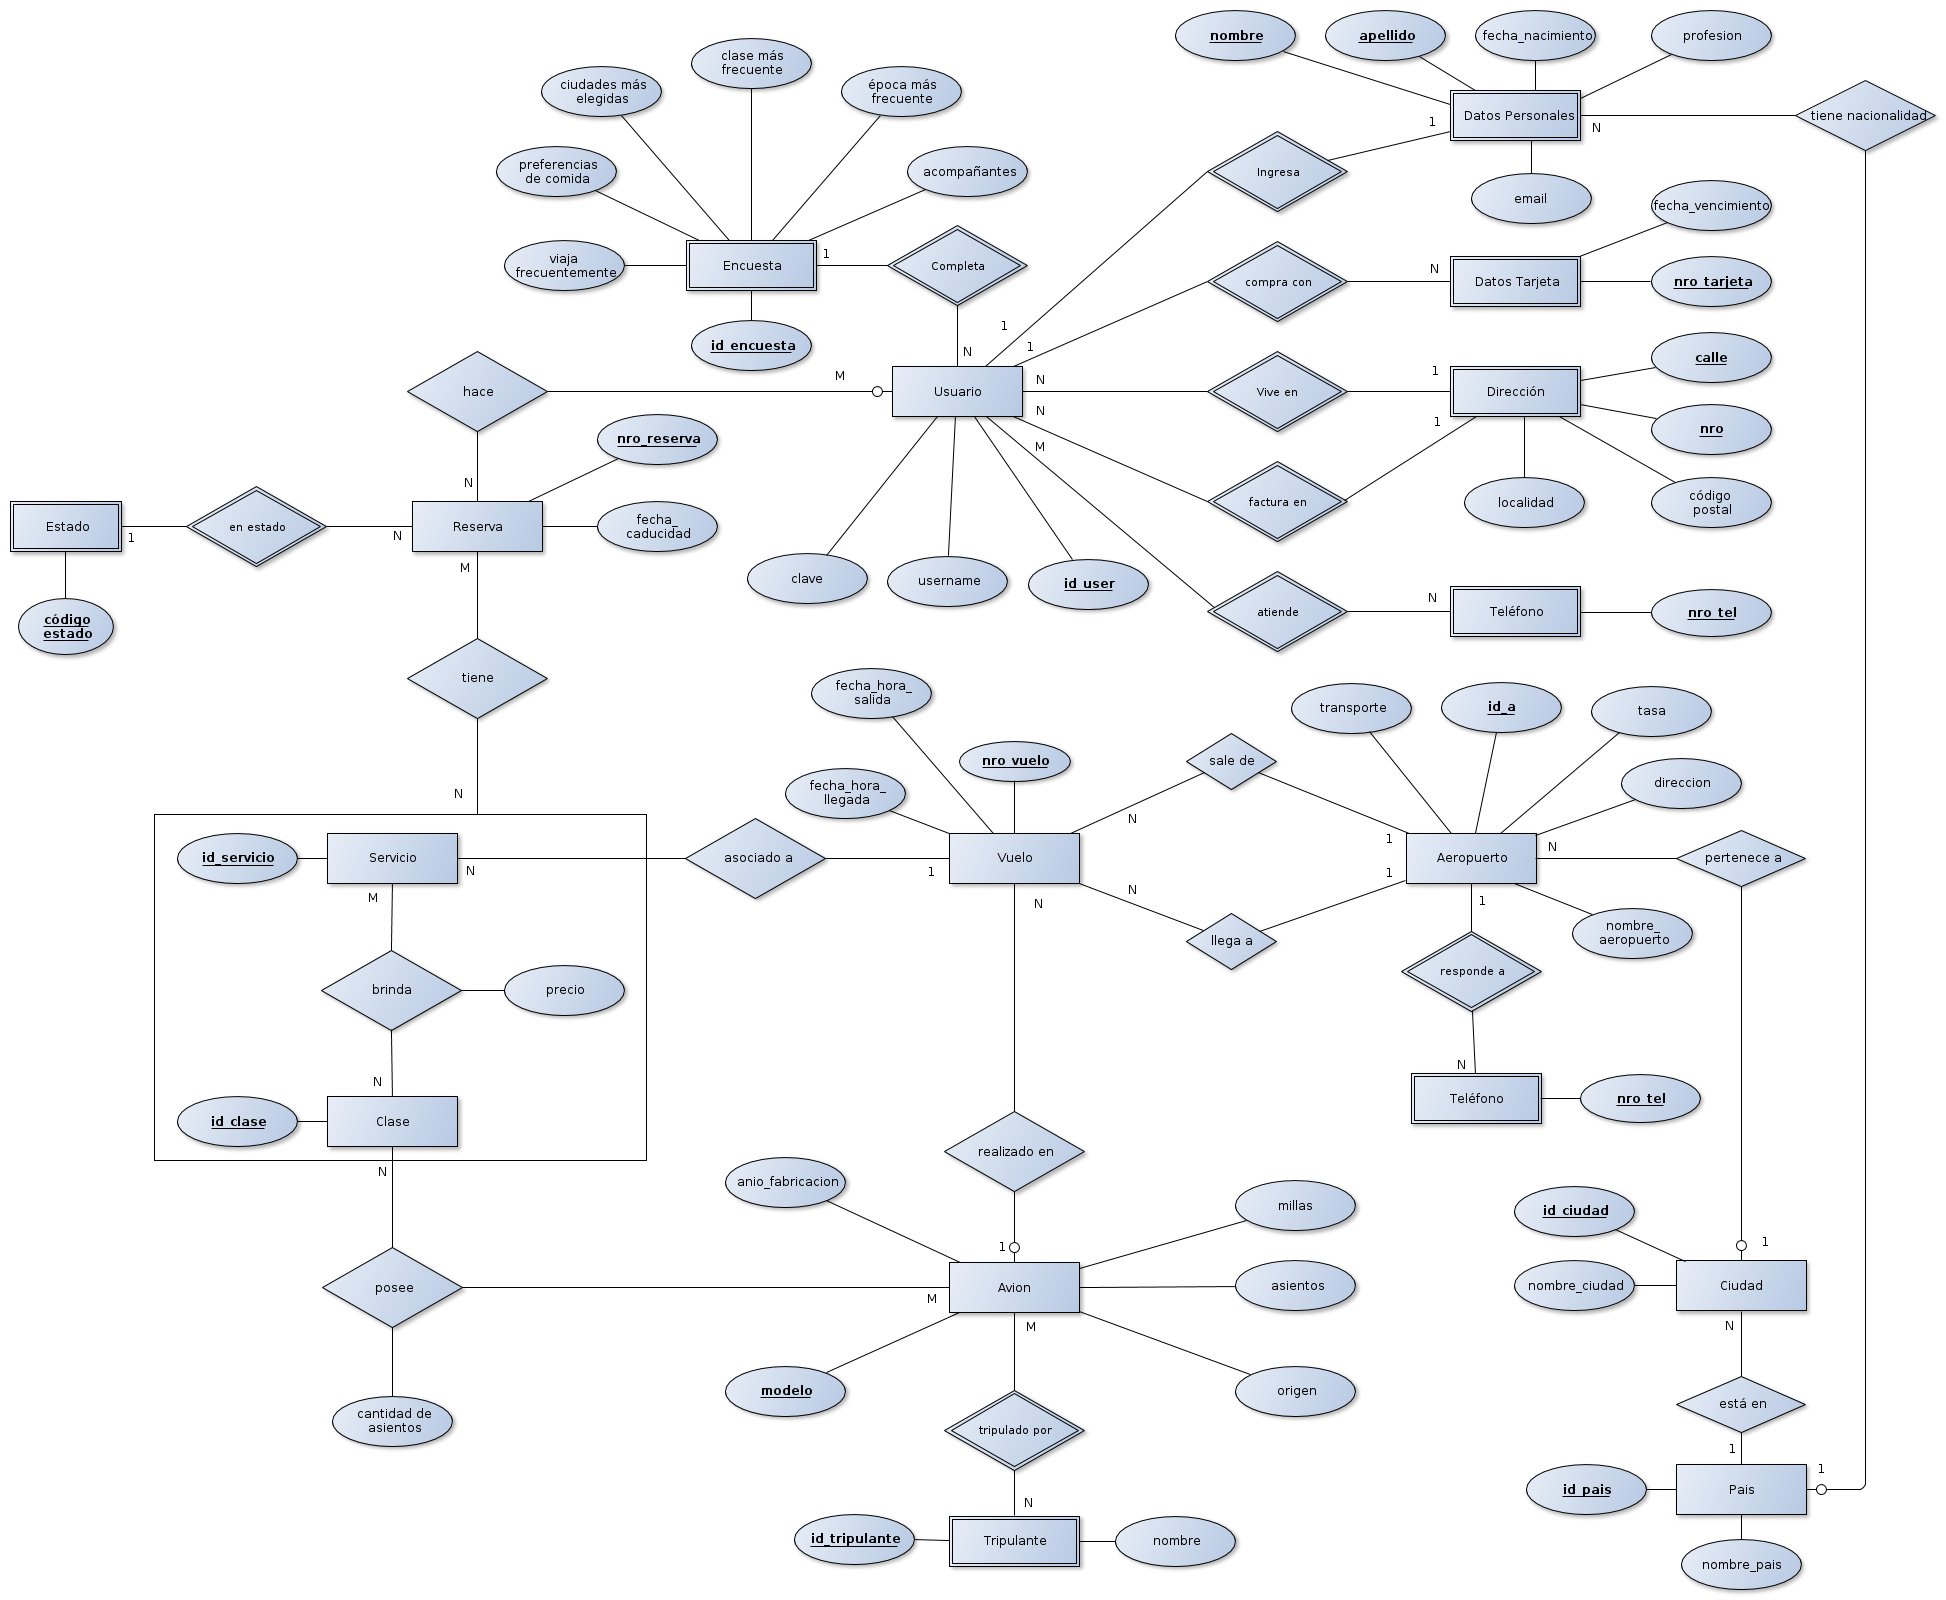
\includegraphics[width=\linewidth]{./img/der.png}}
    {}
  %\hspace*{6cm}
  \end{figure} 

% -----------------------------------------------------------------------------

\subsection{Aclaraciones y Restricciones}
  \begin{itemize}
    \item Consideramos que una reserva puede tener varios estados, estos son
          \begin{itemize}
            \item   Realizada
            \item   Cancelada
            \item   Confirmada
          \end{itemize}

          Las reservas realizadas pueden cancelarse o confirmarse.
          Es necesario confirmar una reserva para poder viajar.
          Para simplificar, suponemos que todos los usuarios con reservas
          confirmadas realizan efectivamente el viaje.
    
    \item La aerolínea ofrece servicios de viaje, y cada usuario realiza una
          reserva sobre pares de servicio-clase.
          De esta forma vemos la cantidad de asientos que está reservando por
          cada clase para un servicio.
          Cada servicio especifica la fecha y el horario del viaje. Además 
          tiene asociado un avión, que es el avión con el que se realizará
          el viaje.
          A la vez un servicio está vinculado con un vuelo. Un vuelo es
          un conjunto de servicios sin especificar. Es decir, un vuelo indica 
          que dias de la semana se brindarán servicios de un aeropuerto origen 
          a uno destino.
          Así, por ejemplo, un servicio podría ser:
          ``Un vuelo de Aeropuerto de origen Ezeiza- Buenos Aires, Aeropuerto 
          destino Newark-New Jersey el día 26/04/2013, 15:00hs, Primera Clas''.
          En cambio, un ejemplo de vuelo es:
         ``Vuelos de Aeropuerto origen Barajas-Madrid, Aeropuerto destino 
          JFK-New York, los días martes y jueve''.
	
    \item Consideramos que los mensajes que el sistema le envía a los usuarios
          no son lo suficientemente relevantes para el problema que queremos
          modelar.
          
    \item Una reserva que se encuentra en estado Realizada, está asociada con un
    	  servicio cuya fecha y hora de salida es anterior a la fecha actual.
    	  
	\item La suma de la cantidad de asientos por clase en un avión (en la 
		  interrelación se distribuyen en) es igual a lo que indica el 
		  atributo asientos de la entidad avión.
	
	\item Este modelo no contempla la posibilidad de que la aerolinea cancele un
		  vuelo. Con lo cual todo vuelo existente es efectuado.
            
  \end{itemize}
	\newpage
	\section{Modelo Relacional}

% Notación
\begin{framed} \centering
  \underline{primary key} \hspace*{3cm}
  \dotuline{foreign key}
\end{framed}

\vspace*{0.5cm}
\noindent
$\mathbf{Usuario}$(\underline{id\_user}, username, clave, nombre, apellido)
\begin{itemize}
	\item $FK = \{(nombre, apellido, calle, nro)\}$
	\item $PK = \{id\_user\}$
	\item $CK = \{id\_user, (nombre, apellido)\}$
	\item $Usuario.nombre$ y $Usuario.apellido$ deben estar en una misma fila
		en $DatosPersonales.nombre$ y $DatosPersonales.apellido$
	\item $Usuario.calle$ y $Usuario.nro$ deben estar en una misma fila
		en $Direccion.calle$ y $Direccion.nro$

\end{itemize}

% Debiles de Usuario

\vspace*{0.5cm}
\noindent
$\mathbf{Encuesta}$(\underline{\dotuline{id\_user}, id\_encuesta},
	viaja\_frecuentemente, preferencias\_de\_comida, ciudades\_elegidas,
	clase\_mas\_frecuente, epoca\_mas\_frecuente, acompaniantes)
\begin{itemize}
	\item $FK = \{id\_user\}$
	\item $PK = CK = \{(id\_user, id\_encuesta)\}$
	\item $Encuesta.id\_user$ debe estar en $Usuario.id\_user$
\end{itemize}

\vspace*{0.5cm}
\noindent
DatosPersonales(\underline{\dotuline{id\_user}, nombre, apellido}, email,
					profesión, fecha\_nacimiento)
\begin{itemize}
	\item $FK = \{id\_user\}$
	\item $PK = CK = \{(id\_user, nombre, apellido\}$
	\item $DatosPersonales.id\_user$ debe estar en $Usuario.id\_user$
\end{itemize}

\vspace*{0.5cm}
\noindent
DatosTarjeta(\underline{\dotuline{id\_user}, nro\_tarjeta}, fecha\_vencimiento)
\begin{itemize}
	\item $FK = \{id\_user\}$
	\item $PK = CK = \{(id\_user, nro\_tarjeta\}$
	\item $DatosTarjeta.id\_user$ debe estar en $Usuario.id\_user$
\end{itemize}

% Como distinguimos las dos relaciones???

\vspace*{0.5cm}
\noindent
Direccion(\underline{\dotuline{id\_user}, calle, nro}, localidad,
					código postal)
\begin{itemize}
	\item $FK = \{id\_user\}$
	\item $PK = CK = \{(id\_user, calle, numero)\}$
	\item $Direccion.id\_user$ debe estar en $Usuario.id\_user$
\end{itemize}

\vspace*{0.5cm}
\noindent
Atiende(\underline{\dotuline{id\_user, nro\_tel}})
\begin{itemize}
	\item $FK = \{id\_user, nro\_tel\}$
	\item $PK = CK = \{(id\_user, nro\_tel)\}$
	\item $Atiende.id\_user$ debe estar en $Usuario.id\_user$
	\item $Atiende.nro\_tel$ debe estar en $Telefono.nro\_tel$
\end{itemize}

\vspace*{0.5cm}
\noindent
Telefono(\underline{\dotuline{id\_user}, nro\_tel})
\begin{itemize}
	\item $FK = \{id\_user\}$
	\item $PK = CK = \{(id\_user, nro\_tel)\}$
	\item $Telefono.id\_user$ debe estar en $Usuario.id\_user$
\end{itemize}


\vspace*{0.5cm}
\noindent
Reserva(\underline{nro\_reserva}, fecha\_caducidad, \dotuline{codigo\_estado})
\begin{itemize}
	\item $FK = \{estado\}$
	\item $PK = CK = \{nro\_reserva\}$
	\item $Reserva.codigo\_estado$ debe estar en $Estado.codigo\_estado$
\end{itemize}

\vspace*{0.5cm}
\noindent
Estado(\underline{codigo\_estado}, descripcion)
\begin{itemize}
	\item $FK = \emptyset$
	\item $PK = CK = \{codigo\_estado\}$
\end{itemize}

\vspace*{0.5cm}
\noindent
Servicio(\underline{id\_servicio}, fecha\_salida, fecha\_llegada,
	hora\_salida, hora\_llegada, \dotuline{nro\_vuelo, modelo})
\begin{itemize}
	\item $FK = \{nro\_vuelo, modelo\}$
	\item $PK = CK = \{id\_servicio\}$
	\item $Servicio.nro\_vuelo$ debe estar en $Vuelo.nro\_vuelo$
	\item $Servicio.modelo$ debe estar en $Avion.modelo$
\end{itemize}

\vspace*{0.5cm}
\noindent
Vuelo(\underline{nro\_vuelo}, \dotuline{aeropuerto\_salida},
	\dotuline{aeropuerto\_llegada})
\begin{itemize}
	\item $FK = \{aeropuerto\_salida, aeropuerto\_llegada\}$
	\item $PK = CK = \{nro\_vuelo\}$
	\item $Vuelo.aeropuerto\_salida$ debe estar en $Aeropuerto.id\_a$
	\item $Vuelo.aeropuerto\_llegada$ debe estar en $Aeropuerto.id\_a$
\end{itemize}

\vspace*{0.5cm}
\noindent
Avion(\underline{modelo}, anio\_fabricacion, millas, asientos, origen)
\begin{itemize}
	\item $FK = \emptyset$
	\item $PK = CK = \{modelo\}$
\end{itemize}


\vspace*{0.5cm}
\noindent
Tripulante(\underline{id\_tripulante}, nombre)
\begin{itemize}
	\item $FK = \emptyset$
	\item $PK = CK = \{id\_tripulante\}$
\end{itemize}


\vspace*{0.5cm}
\noindent
TripuladoPor(\underline{id\_tripulante, modelo})
\begin{itemize}
	\item $FK = \{id\_tripulante, modelo\}$
	\item $PK = CK = \{(id\_tripulante, modelo)\}$
	\item $TripuladoPor.id\_tripulante$ debe estar en
		$Tripulante.id\_tripulante$
	\item $TripuladoPor.modelo$ debe estar en $Avion.modelo$
\end{itemize}

\vspace*{0.5cm}
\noindent
Pais(\underline{id\_pais}, nombre\_pais)
\begin{itemize}
	\item $FK = \emptyset$
	\item $PK = CK = \{id\_pais\}$
\end{itemize}


\vspace*{0.5cm}
\noindent
Ciudad(\underline{id\_ciudad}, nombre\_ciudad, \dotuline{id\_pais})
\begin{itemize}
	\item $FK = \{id\_pais\}$
	\item $PK = CK = \{id\_ciudad\}$
	\item $Ciudad.id\_pais$ debe estar en $Pais.id\_pais$
\end{itemize}

\vspace*{0.5cm}
\noindent
TelefonoAeropuerto(\underline{nro\_tel, \dotuline{id\_a}})
\begin{itemize}
	\item $FK = \{id\_a\}$
	\item $PK = CK = \{(nro\_tel, id\_a\}$
	\item $TelefonoAeropuerto.id\_a$ debe estar en $Aeropuerto.id\_a$
\end{itemize}


\vspace*{0.5cm}
\noindent
Aeropuerto(\underline{id\_a}, tasa, direccion, transporte, nombre\_aeropuerto,
	\dotuline{id\_ciudad})
\begin{itemize}
	\item $FK = \{id\_ciudad\}$
	\item $PK = CK = \{id\_a\}$
	\item $Aeropuerto.id\_ciudad$ debe estar en $Ciudad.id\_ciudad$
\end{itemize}

% \newpage
\subsection{Restricciones}
\begin{itemize}
  \item
  
  \item
\end{itemize}

\subsection{Aclaraciones}
\begin{itemize}
  \item

\end{itemize}

	%\newpage
	\section{Suposiciones Generales}
	\begin{itemize}
    \item     

    \item  

	\end{itemize}

	% \newpage
	% %\section{Modelo F\'isico - Funcionalidades Implementadas}
\section{Modelo F\'isico}

\noindent
Para el modelo f\'isico elegimos utilizar 
% my-sql en un servidor online, que usa php.

\section{Modelo F\'isico - Funcionalidades Pedidas}

%\subsection{Restricciones}
%\subsection{Funcionalidades Implementadas}

\subsection{Stored Procedures}

\noindent
Para ejecutar el c\'odigo de los stored procedures se realiza lo siguiente

\vspace*{0.5cm}
\noindent
\textbf{Ejercicio 1} call ejercicio\_1 ()\\
\textbf{Ejercicio 2} call ejercicio\_2()\\
\textbf{Ejercicio 3} call ...

\newpage
\subsubsection{Proc 1.}

\begin{verbatim}
delimiter $$
create procedure ejercicio_1()
begin

end;
$$
delimiter ;
\end{verbatim}

\vspace*{0.5cm}
\noindent
Aclaraciones .......


\newpage
\subsubsection{Proc 2.}

\begin{verbatim}
delimiter $$
create procedure ejercicio_2()
begin

end;
$$
delimiter ;
\end{verbatim}

\newpage
\subsection{Triggers - Restricciones}

\subsubsection{}

\begin{verbatim}
delimiter $$
create trigger nombre
before insert 
begin

end;
$$
delimiter ;
\end{verbatim}

	% \newpage
	% \section{Modelo F\'isico - Funcionalidades Adicionales}

%\newpage
\subsection{Triggers - Restricciones}
\subsubsection{Trigger 1.}

\begin{verbatim}
delimiter $$
create trigger nombre
before insert 
begin

end;
$$
delimiter ;
\end{verbatim}

\subsubsection{Trigger 2.}
 
\begin{verbatim}
delimiter $$
create trigger nombre
before insert 
begin

end;
$$
delimiter ;
\end{verbatim}
	% \newpage
	% \section{Dificultades Encontradas}

\noindent
% Al encarar el desarrollo de las restricciones del modelo f\'isico, 
% nos encontramos que my-sql tiene algunas limitaciones.

\vspace*{0.5cm}
\noindent
% No permite devolver m\'ultiples filas para un store procedure.
% S\'olo permite un trigger para una misma acci\'on para una misma tabla.

	% \section{Conclusiones}



\end{document}